\documentclass[10pt]{article}

\usepackage[a4paper,margin=0.65in]{geometry}
\usepackage{amsmath,amssymb}
\usepackage{graphicx}
\usepackage{booktabs}
\usepackage{array}
\usepackage{float}
\usepackage{hyperref}
\usepackage{enumitem}
\usepackage{xcolor}
\usepackage{tikz}
\usetikzlibrary{positioning,arrows.meta,shapes.geometric}

\setlist{nosep,leftmargin=*}
\renewcommand{\arraystretch}{1.2}
\setlength{\parindent}{0pt}
\setlength{\parskip}{2pt}

\tikzset{
layer/.style={
draw,
rounded corners,
minimum width=1.5cm,
minimum height=0.6cm,
align=center,
fill=blue!10,
font=\scriptsize
},
att/.style={
draw,
rounded corners,
minimum width=1.5cm,
minimum height=0.6cm,
align=center,
fill=green!12,
font=\scriptsize
},
arrow/.style={
-{Latex[length=2mm]},
thin
}
}

\begin{document}

%%%%%%%%%%%%%%%%%%%%%%%%%%%%%%%%%%%%%%%%%%%%%%%%%%%%%%%%%%%%
% TITLE
%%%%%%%%%%%%%%%%%%%%%%%%%%%%%%%%%%%%%%%%%%%%%%%%%%%%%%%%%%%%

\begin{center}

{\large\textbf{Shiv Nadar University Chennai}}

\vspace{2mm}

{\normalsize\textbf{CS3807 -- Deep Learning Laboratory}}

\vspace{2mm}

{\large\textbf{Experiments 8, 9}}

\vspace{1mm}

{\normalsize\textbf{Effect of Attention Type and Attention Position}}

{\normalsize\textbf{in a Pretrained ResNet50}}

\end{center}

\vspace{3mm}

\begin{tabular}{|p{3.4cm}|p{9.0cm}|p{1.4cm}|}
\hline
Degree \& Branch &
B.Tech Artificial Intelligence \& Data Science &
Semester V\\
\hline
Subject Code \& Name &
CS3807 -- Deep Learning Laboratory &
AY: 2026--27\\
\hline
Name & Madhav.S & \\
\hline
Section & AIDS `B' & \\
\hline
Register Number & 24011101066 & \\
\hline
\end{tabular}

%%%%%%%%%%%%%%%%%%%%%%%%%%%%%%%%%%%%%%%%%%%%%%%%%%%%%%%%%%%%
\section*{1. Objective}

The objective of this experiment is to understand how different attention
mechanisms modify a pretrained convolutional network, and how the
\textbf{position at which attention is inserted} influences image
classification performance.

A single backbone, ResNet50 pretrained on ImageNet, was used throughout on
the TensorFlow Flowers dataset (five classes). Channel, spatial, sequential
channel--spatial, lightweight self-attention, ECA and CBAM modules were
inserted at different stages and compared quantitatively (accuracy,
precision, recall, macro F1, parameters, inference time) and qualitatively
(internal attention maps and Grad-CAM).

%%%%%%%%%%%%%%%%%%%%%%%%%%%%%%%%%%%%%%%%%%%%%%%%%%%%%%%%%%%%
\section*{2. Learning Outcomes}

After completing this experiment, students will be able to:

\begin{itemize}
\item explain the stage-wise architecture of a pretrained ResNet50;
\item distinguish early, intermediate, and late convolutional features;
\item explain the motivation behind attention mechanisms;
\item implement channel, spatial, sequential channel--spatial and lightweight self-attention;
\item insert an attention module at different stages of a pretrained network;
\item analyze the influence of attention position;
\item compare different attention mechanisms under a controlled experimental protocol;
\item analyze classification accuracy and class-wise performance;
\item visualize internal attention maps and generate Grad-CAM explanations;
\item distinguish an internal attention map from a post-hoc explanation map;
\item analyze accuracy--complexity trade-offs; and
\item perform controlled ablation studies.
\end{itemize}

%%%%%%%%%%%%%%%%%%%%%%%%%%%%%%%%%%%%%%%%%%%%%%%%%%%%%%%%%%%%
\section*{3. Dataset and Experimental Setup}

\textbf{Dataset: TensorFlow Flowers (\texttt{tf\_flowers})}

The dataset contains 3{,}670 natural RGB flower images in five classes:
daisy, dandelion, roses, sunflowers and tulips. Every image was resized to

\[
224\times224\times3
\]

and preprocessed with ResNet50's own \texttt{preprocess\_input} function.
Random horizontal flip, small rotation, random zoom, random translation and
mild contrast variation were applied to the \emph{training set only}, and
the same augmentation was used for every model.

\textbf{Split.} The images were split by class (stratified) into a fixed
70/15/15 train/validation/test split using seed 42. The exact same samples
were used in every experiment.

\begin{center}
\small
\begin{tabular}{|l|c|c|c|c|c|c|}
\hline
Split & Images & Daisy & Dandelion & Roses & Sunflowers & Tulips\\
\hline
Training & 2{,}569 & 443 & 629 & 449 & 489 & 559\\
Validation & 550 & 95 & 134 & 96 & 105 & 120\\
Test & 551 & 95 & 135 & 96 & 105 & 120\\
\hline
\end{tabular}
\end{center}

\begin{center}
\includegraphics[width=0.5\linewidth]{fig01_sample_images.pdf}
\end{center}

\textbf{Inference:} The samples show how varied the data is: single close-ups
and whole fields, bright and dark scenes, cluttered backgrounds, and even
people in the frame (sunflower and tulip rows). Some roses (pink bouquets)
and tulips share similar colours and rounded petals, so these two classes
are the likeliest to be confused later on.

%%%%%%%%%%%%%%%%%%%%%%%%%%%%%%%%%%%%%%%%%%%%%%%%%%%%%%%%%%%%
\section*{4. ResNet50 Architecture and Attention Positions}

ResNet50 pretrained on ImageNet is the only backbone. As the network gets
deeper the spatial resolution falls while the number of channels grows, and
the features move from edges and textures to high-level, class-specific
semantics. The stage dimensions below were verified on the Keras model:

\begin{center}
\begin{tabular}{|l|c|c|c|c|}
\hline
ResNet50 Stage & Spatial Resolution & Channels & Position & Feature Type\\
\hline
Stem + MaxPool & $56\times56$ & 64 & -- & early\\
conv2\_x & $56\times56$ & 256 & $P_1$ & early\\
conv3\_x & $28\times28$ & 512 & $P_2$ & intermediate\\
conv4\_x & $14\times14$ & 1024 & $P_3$ & intermediate\\
conv5\_x & $7\times7$ & 2048 & $P_4$ & late / semantic\\
\hline
\end{tabular}
\end{center}

For any selected stage $P_k$ the network becomes
\emph{Previous ResNet Stage $\rightarrow$ Attention $\rightarrow$ Next ResNet Stage},
followed by Global Average Pooling, Dropout (0.3) and a Dense layer with 5
softmax neurons. The input and output dimensions of every attention block
were recorded and were identical (for example $14\times14\times1024$
before and after attention at $P_3$), so attention never changed the
feature size.

\begin{center}
\resizebox{\linewidth}{!}{%
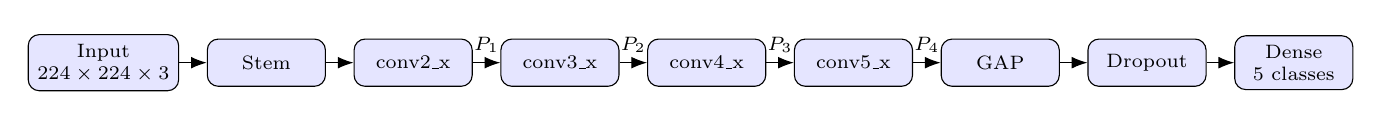
\begin{tikzpicture}[node distance=3.5mm]

\node[layer](a){Input\\$224\times224\times3$};
\node[layer,right=of a](b){Stem};
\node[layer,right=of b](c){conv2\_x};
\node[layer,right=of c](d){conv3\_x};
\node[layer,right=of d](e){conv4\_x};
\node[layer,right=of e](f){conv5\_x};
\node[layer,right=of f](g){GAP};
\node[layer,right=of g](h){Dropout};
\node[layer,right=of h](i){Dense\\5 classes};

\foreach \x/\y in {a/b,b/c,g/h,h/i}
\draw[arrow](\x)--(\y);

\draw[arrow](c)--node[above,font=\scriptsize]{$P_1$}(d);
\draw[arrow](d)--node[above,font=\scriptsize]{$P_2$}(e);
\draw[arrow](e)--node[above,font=\scriptsize]{$P_3$}(f);
\draw[arrow](f)--node[above,font=\scriptsize]{$P_4$}(g);

\end{tikzpicture}}
\end{center}

\textbf{Note:} Attention modules are inserted at the positions marked
$P_1$--$P_4$. $P_3$ is the fixed position for the attention-type study
(Experiment 1).

%%%%%%%%%%%%%%%%%%%%%%%%%%%%%%%%%%%%%%%%%%%%%%%%%%%%%%%%%%%%
\section*{5. Attention Mechanisms}

Every module takes $F\in\mathbb{R}^{H\times W\times C}$ and returns a tensor
of the same shape.

\textbf{Channel attention} (``which channels are important?''), with
reduction ratio $r=16$:

\[
z_c=\frac{1}{HW}\sum_{i=1}^{H}\sum_{j=1}^{W}F(i,j,c),\qquad
M_c(F)=\sigma\left(W_2\,\delta(W_1 z)\right),\qquad
F_c=F\odot M_c(F).
\]

\textbf{Spatial attention} (``which locations are important?''), kernel $7\times7$:

\[
F_s=[\mathrm{Mean}_c(F)\,\|\,\mathrm{Max}_c(F)],\qquad
M_s(F)=\sigma\left(\mathrm{Conv}_{7\times7}(F_s)\right),\qquad
F_s'=F\odot M_s(F).
\]

\textbf{Sequential channel--spatial attention:}
$F_c=M_c(F)\odot F$, then $F_{cs}=M_s(F_c)\odot F_c$. The reverse order
(spatial first) was used for Experiment 4.

\textbf{Lightweight self-attention:} with $X\in\mathbb{R}^{N\times C}$,
$N=HW$, $Q=XW_Q$, $K=XW_K$, $V=XW_V$,

\[
A=\mathrm{softmax}\!\left(\frac{QK^{T}}{\sqrt{d}}\right),\qquad
Y=AV,\qquad
F_{SA}=F+\gamma\,\mathrm{reshape}(Y),
\]

where $\gamma$ is a learnable scale initialised to 0 and $d=C/8$ is the
query/key size. \textbf{Combined attention} (A5) applies channel, spatial
and self-attention one after another.

\textbf{Additional mechanisms.} \emph{ECA} replaces the two dense layers of
channel attention by a single 1-D convolution across neighbouring channels
(kernel size 5 for 1024 channels, no dimensionality reduction).
\emph{CBAM} computes channel attention from both average- and max-pooled
descriptors through a shared MLP, followed by $7\times7$ spatial attention.
The channel-attention module above is the Squeeze-and-Excitation (SE)
formulation, so ``Channel'' and ``SE'' refer to the same model in all
tables and plots.

%%%%%%%%%%%%%%%%%%%%%%%%%%%%%%%%%%%%%%%%%%%%%%%%%%%%%%%%%%%%
\section*{6. Training Protocol and Evaluation}

\begin{center}
\begin{tabular}{|l|p{11.5cm}|}
\hline
Item & Setting (identical for every model)\\
\hline
Backbone & ResNet50, ImageNet weights, original classifier removed\\
Classifier & Global Average Pooling $\rightarrow$ Dropout (0.3) $\rightarrow$ Dense (5, softmax)\\
Stage 1 & backbone frozen; attention and classifier trained, Adam, LR $=10^{-3}$, 10 epochs\\
Stage 2 & conv5\_x unfrozen (BatchNorm layers kept frozen), Adam, LR $=10^{-4}$, 10 epochs\\
Other & batch size 32, categorical cross-entropy, random seed 42, NVIDIA Tesla T4 GPU\\
\hline
\end{tabular}
\end{center}

Accuracy, macro precision, macro recall and macro F1 were computed on the
test set, with $\mathrm{Macro\ F1}=\frac{1}{C}\sum_{c=1}^{C}F1_c$ and
$C=5$. Trainable parameters are counted in the fine-tuning state (attention
+ conv5\_x + classifier), total parameters include the whole network, and
inference time is the average time per image over the test set (batches of 32).
Since the test set has 551 images, \textbf{one image equals about 0.18
percentage points}; differences of a few images are within what a re-run
could change.

%%%%%%%%%%%%%%%%%%%%%%%%%%%%%%%%%%%%%%%%%%%%%%%%%%%%%%%%%%%%
\section*{7. Experiment 1: Attention-Type Ablation (Position $P_3$)}

\begin{center}
\small
\begin{tabular}{|l|c|c|c|c|c|c|}
\hline
Model & Acc. (\%) & Precision & Recall & Macro F1 & Parameters & Time (ms)\\
\hline
A0: Baseline ResNet50 & \textbf{94.37} & 0.9465 & 0.9421 & 0.9436 & 23{,}597{,}957 & 7.67\\
A1: Channel Attention & 93.47 & 0.9373 & 0.9316 & 0.9339 & 23{,}730{,}117 & 7.66\\
A2: Spatial Attention & 93.65 & 0.9411 & 0.9338 & 0.9368 & 23{,}598{,}056 & 8.42\\
A3: Channel+Spatial & 93.83 & 0.9413 & 0.9357 & 0.9370 & 23{,}730{,}216 & 7.70\\
A4: Self-Attention & 94.19 & 0.9453 & 0.9387 & 0.9410 & 24{,}908{,}678 & 8.20\\
A5: Combined Attention & 91.65 & 0.9181 & 0.9139 & 0.9154 & 25{,}040{,}937 & 7.74\\
\hline
\end{tabular}
\end{center}

\textbf{Inference:} None of the attention variants beat the plain ResNet50.
Self-attention comes closest (one image fewer than the baseline), and the
single modules (A1--A3) are about 0.5--0.9 points below it. The clear
outlier is the combined model A5, which combines the three modules, adds 1.44M
parameters and loses 2.7 points (505 versus 520 correct images). With only
2{,}569 training images, a bigger attention block seems to give the network
more to overfit rather than more to use.

%%%%%%%%%%%%%%%%%%%%%%%%%%%%%%%%%%%%%%%%%%%%%%%%%%%%%%%%%%%%
\section*{8. Experiment 2: Attention-Position Ablation (Channel $\rightarrow$ Spatial)}

\begin{center}
\small
\begin{tabular}{|l|c|c|c|c|c|c|c|}
\hline
Experiment & Resolution & Acc. (\%) & Precision & Recall & Macro F1 & Parameters & Time (ms)\\
\hline
B1: after conv2\_x ($P_1$) & $56\times56\times256$ & 92.56 & 0.9245 & 0.9271 & 0.9252 & 23{,}606{,}520 & 8.40\\
B2: after conv3\_x ($P_2$) & $28\times28\times512$ & 92.20 & 0.9263 & 0.9196 & 0.9206 & 23{,}631{,}368 & 8.37\\
B3: after conv4\_x ($P_3$) & $14\times14\times1024$ & \textbf{93.83} & 0.9413 & 0.9357 & 0.9370 & 23{,}730{,}216 & 7.70\\
B4: after conv5\_x ($P_4$) & $7\times7\times2048$ & 93.65 & 0.9405 & 0.9369 & 0.9367 & 24{,}124{,}520 & 8.41\\
\hline
\end{tabular}
\end{center}

\textbf{Inference:} The middle-to-late positions work best: $P_3$ is on top
(93.83\%) with $P_4$ right behind (93.65\%), while the early positions $P_1$
and $P_2$ are 1.3--1.6 points lower. Early features are edges and textures
that are all useful, so there is little for attention to select, whereas
deeper features are more class-specific. $P_4$ also costs four times as
many extra parameters as $P_3$ (526{,}563 versus 132{,}259) because it
works on 2048 channels, for no gain, so $P_3$ is the best trade-off here.

%%%%%%%%%%%%%%%%%%%%%%%%%%%%%%%%%%%%%%%%%%%%%%%%%%%%%%%%%%%%
\section*{9. Experiment 3: Multiple Attention Positions (Channel $\rightarrow$ Spatial)}

\begin{center}
\small
\begin{tabular}{|l|c|c|c|c|c|c|}
\hline
Model & Acc. (\%) & Macro F1 & Added params & Train (s) & Peak GPU (MB) & Inf. (ms)\\
\hline
Only $P_3$ & \textbf{93.83} & 0.9370 & 132{,}259 & 858 & 1{,}322 & 7.70\\
Only $P_4$ & 93.65 & 0.9367 & 526{,}563 & 848 & 2{,}577 & 8.41\\
$P_3+P_4$ & 93.47 & 0.9346 & 658{,}822 & 862 & 2{,}801 & 8.56\\
$P_2+P_3+P_4$ (extended) & 93.47 & 0.9346 & 692{,}233 & 867 & 3{,}409 & 8.69\\
\hline
\end{tabular}
\end{center}

\textbf{Inference:} Adding attention at more stages did not help. Accuracy
drifts down from 93.83\% to 93.47\% (two images) while the extra
parameters grow five-fold, GPU memory rises from about 1.3~GB to
3.4~GB and inference time goes up by about 1~ms. Training time barely
changes (around 14 minutes for every model). So attention at more locations is not necessarily more
effective, and the single $P_3$ module gives the best return.
%%%%%%%%%%%%%%%%%%%%%%%%%%%%%%%%%%%%%%%%%%%%%%%%%%%%%%%%%%%%
\section*{10. Experiment 4: Attention Order (at $P_3$)}

\begin{center}
\small
\begin{tabular}{|l|c|c|c|c|c|}
\hline
Order & Acc. (\%) & Precision & Recall & Macro F1 & Time (ms)\\
\hline
Channel $\rightarrow$ Spatial ($F\rightarrow M_c\rightarrow M_s$) & 93.83 & 0.9413 & 0.9357 & 0.9370 & 7.70\\
Spatial $\rightarrow$ Channel ($F\rightarrow M_s\rightarrow M_c$) & 93.83 & 0.9407 & 0.9395 & 0.9396 & 8.27\\
\hline
\end{tabular}
\end{center}

\textbf{Inference:} The order made no real difference: accuracy is
identical, and spatial-first has a slightly better recall and macro F1
(+0.26 points, about one or two images). Both models have exactly the same
parameters (23{,}730{,}216) and perform the same operations, yet their
timings differ by 0.6~ms, which shows that timing gaps below about 1~ms in
this report are measurement noise rather than real cost.

%%%%%%%%%%%%%%%%%%%%%%%%%%%%%%%%%%%%%%%%%%%%%%%%%%%%%%%%%%%%
\section*{11. Experiment 5: Spatial-Attention Kernel Size (at $P_3$)}

\begin{center}
\begin{tabular}{|c|c|c|c|}
\hline
Spatial Kernel & Accuracy (\%) & Macro F1 & Inference Time (ms)\\
\hline
$3\times3$ & 92.01 & 0.9157 & 8.30\\
$5\times5$ & 93.10 & 0.9321 & 8.35\\
$7\times7$ & \textbf{93.65} & \textbf{0.9368} & 8.42\\
\hline
\end{tabular}
\end{center}

\textbf{Inference:} Accuracy and macro F1 both rise steadily with the
kernel size, from 92.01\% to 93.65\% (nine more images correct). A
$3\times3$ window only sees a tiny part of the $14\times14$ map, while a
$7\times7$ window collects much greater context before deciding which
locations matter. The price is negligible (about 80 more parameters and
0.1~ms), so a larger kernel is a useful increase in context here.

%%%%%%%%%%%%%%%%%%%%%%%%%%%%%%%%%%%%%%%%%%%%%%%%%%%%%%%%%%%%
\section*{12. Additional Task: Comparison of Attention Mechanisms (at $P_3$)}

ECA and CBAM were added as established mechanisms and compared with the
modules above, all on the same ResNet50 and inserted at $P_3$. The last
column gives the parameters each module adds to the baseline.

\begin{center}
\small
\begin{tabular}{|l|c|c|c|c|c|c|}
\hline
Attention & Acc. (\%) & Precision & Recall & Macro F1 & Params added & Time (ms)\\
\hline
No Attention & 94.37 & 0.9465 & 0.9421 & 0.9436 & 0 & 7.67\\
Channel / SE & 93.47 & 0.9373 & 0.9316 & 0.9339 & 132{,}160 & 7.66\\
Spatial Attention & 93.65 & 0.9411 & 0.9338 & 0.9368 & 99 & 8.42\\
\textbf{ECA} & \textbf{94.56} & \textbf{0.9480} & \textbf{0.9443} & \textbf{0.9459} & 5 & 8.33\\
CBAM & 94.37 & 0.9462 & 0.9439 & 0.9444 & 132{,}259 & 8.39\\
Self-Attention & 94.19 & 0.9453 & 0.9387 & 0.9410 & 1{,}310{,}721 & 8.20\\
\hline
\end{tabular}
\end{center}

\textbf{Inference:} ECA is the best model on every quality metric and also
the cheapest, adding just 5 parameters, although its lead over the
baseline is a single image (521 versus 520). CBAM ties the baseline,
SE is the weakest, and self-attention, with 1.31M extra parameters, ends
below the baseline. The lightweight mechanism therefore matches or beats
the heavier ones, and more parameters did not mean higher accuracy.

%%%%%%%%%%%%%%%%%%%%%%%%%%%%%%%%%%%%%%%%%%%%%%%%%%%%%%%%%%%%
\section*{13. Required Main Result Table}

\begin{center}
\small
\begin{tabular}{|l|c|c|c|c|c|c|c|}
\hline
Model & Position & Acc. (\%) & Precision & Recall & F1 & Parameters & Time (ms)\\
\hline
Baseline & -- & 94.37 & 0.9465 & 0.9421 & 0.9436 & 23{,}597{,}957 & 7.67\\
Channel Attention & $P_3$ & 93.47 & 0.9373 & 0.9316 & 0.9339 & 23{,}730{,}117 & 7.66\\
Spatial Attention & $P_3$ & 93.65 & 0.9411 & 0.9338 & 0.9368 & 23{,}598{,}056 & 8.42\\
Channel+Spatial & $P_2$ & 92.20 & 0.9263 & 0.9196 & 0.9206 & 23{,}631{,}368 & 8.37\\
Channel+Spatial & $P_3$ & 93.83 & 0.9413 & 0.9357 & 0.9370 & 23{,}730{,}216 & 7.70\\
Channel+Spatial & $P_4$ & 93.65 & 0.9405 & 0.9369 & 0.9367 & 24{,}124{,}520 & 8.41\\
Self-Attention & $P_3$ & 94.19 & 0.9453 & 0.9387 & 0.9410 & 24{,}908{,}678 & 8.20\\
Additional Attention-1 (ECA) & $P_3$ & \textbf{94.56} & 0.9480 & 0.9443 & 0.9459 & 23{,}597{,}962 & 8.33\\
Additional Attention-2 (CBAM) & $P_3$ & 94.37 & 0.9462 & 0.9439 & 0.9444 & 23{,}730{,}216 & 8.39\\
\hline
\end{tabular}
\end{center}

The trainable parameters (attention + conv5\_x + classifier) range from
14{,}963{,}717 for the baseline to 16{,}274{,}438 for self-attention.

%%%%%%%%%%%%%%%%%%%%%%%%%%%%%%%%%%%%%%%%%%%%%%%%%%%%%%%%%%%%
\section*{14. Graphical Performance Analysis}

\begin{center}
\includegraphics[width=0.95\linewidth]{fig02_accuracy_curves.pdf}
\end{center}

\textbf{Inference:} All models learn in the same way: a fast rise during
the frozen stage, a dip when conv5\_x is unfrozen at epoch 11, and
98--99\% training accuracy by epoch 16. Self-attention starts fastest
(about 89\% training accuracy after epoch 2) and ECA slowest (about 76\%),
but by epoch 12 they are level. Validation accuracy stays in the
91--95\% band and is noisy during fine-tuning (Channel+Spatial and CBAM
dip to about 89\% at times). The train--validation gap stays near 5 points
for most models (for example, 98.9\% versus 94.0\% for the baseline), so
attention did not speed up convergence, smooth learning or reduce
overfitting.

\begin{center}
\includegraphics[width=0.95\linewidth]{fig03_loss_curves.pdf}
\end{center}

\textbf{Inference:} Training loss falls from 0.7--1.2 to about 0.03--0.07,
with a short jump when fine-tuning starts. Validation loss, however,
settles at 0.25--0.40 after the first few epochs and never improves
further, which is the usual sign of overfitting, and it has spikes after
fine-tuning (Spatial at epoch 19, CBAM at epoch 17). Self-attention has the
lowest training loss early on but the highest final validation loss
(0.43), so it fits the training set fastest but generalizes no better.

\begin{center}
\includegraphics[width=0.48\linewidth]{fig04_attention_vs_accuracy.pdf}
\hfill
\includegraphics[width=0.48\linewidth]{fig05_attention_vs_macro_f1.pdf}
\end{center}

\textbf{Inference:} ECA is highest in both plots (94.56\% accuracy, 0.946
macro F1), the baseline and CBAM tie on accuracy, and SE is lowest. The
whole spread is only about 1.1 points (six images), and the macro F1
ranking follows the accuracy ranking, so no mechanism gives a clear
improvement over the baseline.

\begin{center}
\includegraphics[width=0.48\linewidth]{fig06_accuracy_vs_parameters.pdf}
\hfill
\includegraphics[width=0.48\linewidth]{fig07_macro_f1_vs_inference_time.pdf}
\end{center}

\textbf{Inference:} Accuracy does not follow the parameter count: the
most expensive point (self-attention, +1.31M) is below the baseline, while
the cheapest (ECA, +5) is the best. In the right plot all models lie within
7.7--8.4~ms and the order does not follow the parameters either (the
99-parameter spatial module is the slowest, SE with 132k parameters is as
fast as the baseline), so these gaps are mostly timing noise. ECA's gain of
0.23 F1 points for 0.65~ms extra is too small to call a real trade-off.

%%%%%%%%%%%%%%%%%%%%%%%%%%%%%%%%%%%%%%%%%%%%%%%%%%%%%%%%%%%%
\section*{15. Confusion Matrix Analysis}

The baseline ResNet50 and the selected attention model (Channel+Spatial at
$P_3$) are compared on the five-class test set.

\begin{center}
\includegraphics[width=0.95\linewidth]{fig08_confusion_matrices.pdf}
\end{center}

\begin{center}
\small
\begin{tabular}{|l|c|c|c|c|c|}
\hline
Class & Support & Recall (Base) & Recall (C+S) & F1 (Base) & F1 (C+S)\\
\hline
Daisy & 95 & 0.9684 & 0.9684 & 0.9684 & 0.9634\\
Dandelion & 135 & 0.9630 & 0.9556 & 0.9524 & 0.9699\\
Roses & 96 & 0.8646 & 0.8333 & 0.9121 & 0.8939\\
Sunflowers & 105 & 0.9810 & 0.9714 & 0.9671 & 0.9533\\
Tulips & 120 & 0.9333 & 0.9500 & 0.9180 & 0.9048\\
\hline
\end{tabular}
\end{center}

\textbf{Inference:} Sunflowers and daisies are classified most accurately,
and roses are clearly the weakest class. The dominant error is roses
predicted as tulips (9 images for the baseline, 14 with attention), which
accounts for nearly all of the attention model's three extra mistakes
(517 versus 520 correct). Only dandelion benefits: far fewer roses and
tulips are wrongly called dandelion (6 to 0), lifting its F1 from 0.952
to 0.970. The other four classes lose 0.5--1.8 F1 points, so the overall
accuracy is not spread evenly.

%%%%%%%%%%%%%%%%%%%%%%%%%%%%%%%%%%%%%%%%%%%%%%%%%%%%%%%%%%%%
\section*{16. Qualitative Analysis of Attention}

An \textbf{internal attention map} is computed by the module during the
forward pass, whereas \textbf{Grad-CAM} is a post-hoc explanation computed
after the prediction from the gradients of the class score,
$L^c_{\text{Grad-CAM}}=\mathrm{ReLU}\left(\sum_k\alpha_k^cA^k\right)$,
taken on the feature map entering global average pooling. The same five
test images were used for every figure: three correctly classified (daisy,
dandelion, rose bouquet) and two misclassified roses (rose buds and a dried
rose bush).

\subsection*{16.1 Feature Maps Before and After Attention}

\begin{center}
\includegraphics[width=0.98\linewidth]{fig09_feature_maps_before_after_attention.pdf}
\end{center}

\textbf{Inference:} The maps at $P_3$ ($14\times14\times1024$) before and
after attention are almost identical. The mean map and the eight strongest
channels keep the same pattern, and only a few channels are slightly dimmed
(for example channel 908). The module therefore changes the features very
little, which agrees with the small accuracy differences.

\subsection*{16.2 Channel-Attention Weights}

\begin{center}
\includegraphics[width=0.9\linewidth]{fig10_channel_attention_weights.pdf}
\end{center}

\textbf{Inference:} In all three images the top-10 channels have weights
of about 1.0, so the sigmoid is saturated. Over 64 test images, the mean
weight is 0.62 and 63\% of all 1024 channels are above 0.5, so many
channels contribute rather than a small handful. 

\subsection*{16.3 Spatial-Attention Map and Overlay}

\begin{center}
\includegraphics[width=0.38\linewidth]{fig11_spatial_attention_map_overlay.pdf}
\end{center}

\textbf{Inference:} After min--max scaling, nearly the whole image sits at
the top of the range (dark red), and the low values (blue) form thin bands
along the bottom, left and top borders. The module has mostly learned to
turn down border cells (possibly zero-padding effects of the $7\times7$
convolution) and not the background around the flower. It therefore does not
single out petals or the flower centre, and the same pattern appears for
correctly and incorrectly classified images.

\subsection*{16.4 Self-Attention Response}

\begin{center}
\includegraphics[width=0.7\linewidth]{fig12_self_attention_response.pdf}
\end{center}

\textbf{Inference:} At $P_3$ the attention matrix is $196\times196$. For
every image the response is one small hotspot on a flower (a single daisy,
the centre of the dandelion, one rose), and the mean and maximum over all
query positions show almost the same spot as the centre query. So every
query attends to nearly the same location instead of to its own related
regions, which means very little interaction between distant parts of the
image and fits the lack of any accuracy gain from self-attention.

\subsection*{16.5 Grad-CAM: Input $|$ Baseline $|$ Attention Model}

\begin{center}
\includegraphics[width=0.38\linewidth]{fig13_gradcam_baseline_vs_attention.pdf}
\end{center}

\textbf{Inference:} For the three correct images, the baseline and
Channel+Spatial maps are nearly the same: weak, spread over the whole
daisies and dandelion, and concentrated on the dark red rose at the right
of the bouquet. For the rose buds both models predict tulips with the
heat on the bud, and the attention model's region is slightly wider. For
the dried rose bush the baseline splits its focus between a left blob and a
branch (predicting dandelion), whereas the attention model puts it on the
left blob (predicting tulips). The small rose cluster in the centre is not
highlighted by either, so the attention model shows no clear improvement in
where the network looks.

\subsection*{16.6 Attention at Different Positions: Input $|$ $M_s^{P_2}$ $|$ $M_s^{P_3}$ $|$ $M_s^{P_4}$}

\begin{center}
\includegraphics[width=0.55\linewidth]{fig14_spatial_attention_positions_P2_P3_P4.pdf}
\end{center}

\textbf{Inference:} The maps become coarser with depth. $M_s^{P_2}$
($28\times28$) is almost uniform apart from a thin low strip at the bottom
edge, $M_s^{P_3}$ ($14\times14$) shows the same bottom strip plus the left
edge and top-left corner, and $M_s^{P_4}$ ($7\times7$) has a few large
blocks at the corners. The expected behaviour (edges and textures at $P_2$,
flower parts at $P_3$, whole flower regions at $P_4$) was not seen.

\subsection*{16.7 Qualitative Comparison Across Attention Mechanisms}

\begin{center}
\includegraphics[width=0.95\linewidth]{fig15_qualitative_comparison_attention_types.pdf}
\end{center}

\textbf{Inference:} For the daisy and dandelion all Grad-CAMs are faint
and cover the whole flower. For the bouquet the baseline and
Channel+Spatial both focus on the red rose, while the channel-only model
shows almost no heat. On the rose buds all three focus on the bud (all
predict tulips), and on the dried rose bush the channel model concentrates
on the central rose cluster but still predicts tulips. Evidence is therefore mostly on
the flower for correct images, and misclassified images fail even when the
heat is on a sensible region.

\begin{center}
\includegraphics[width=0.95\linewidth]{fig16_qualitative_comparison_additional_mechanisms.pdf}
\end{center}

\textbf{Inference:} ECA classifies both difficult images correctly (rose
buds and dried rose bush) and CBAM gets the dried rose bush right, while
baseline and SE get both wrong. For the dried rose bush CBAM concentrates
its heat on the rose cluster, whereas ECA's heat is spread over branches
and the bottom-right, so it is right with weaker localization. With only
five images this is an observation, but it matches ECA's slight
lead in the tables.

%%%%%%%%%%%%%%%%%%%%%%%%%%%%%%%%%%%%%%%%%%%%%%%%%%%%%%%%%%%%
\section*{17. Discussion Questions}

\begin{enumerate}
\item \textbf{What is the purpose of residual connections in ResNet50?}
They add a block's input to its output, giving gradients a direct path
backwards. This lets very deep networks train without vanishing gradients
or degradation.

\item \textbf{What does conv2\_x represent compared with conv5\_x?}
conv2\_x is the first stage ($56\times56\times256$) and holds early
features such as edges and textures. conv5\_x is the last stage
($7\times7\times2048$) and holds high-level, class-discriminative
information.

\item \textbf{Why does the spatial resolution decrease with network depth?}
Strided convolutions and pooling downsample the feature maps. This grows
the receptive field, reduces computation, and makes features more abstract.

\item \textbf{Why does the number of feature channels increase with network depth?}
As spatial detail shrinks, more filters are needed to represent the growing
variety of patterns, and it keeps the computation per stage balanced.

\item \textbf{What is meant by low-level, intermediate, and high-level features?}
Low-level features are edges, colours and simple textures. Intermediate
features are local patterns, petal arrangements and shapes. High-level
features are object structures and class-specific semantics.

\item \textbf{What is the purpose of an attention mechanism?}
To let the network emphasize the useful channels or locations and
suppress the less useful ones before passing features on.

\item \textbf{What does channel attention attempt to learn?}
Which feature channels are important, as a weight $m_c$ for each channel
computed from the globally pooled descriptor.

\item \textbf{What does spatial attention attempt to learn?}
Which spatial locations are important, as an $H\times W$ weight map.

\item \textbf{How is channel attention different from spatial attention?}
Channel attention rescales whole channels using one weight per channel
(the same at every location). Spatial attention rescales locations using one
weight per position (the same for every channel).

\item \textbf{Why can channel and spatial attention be used sequentially?}
They act on different dimensions, so the first decides ``what'' is
important and the second ``where''. In Experiment 4 either order gave
93.83\% accuracy.

\item \textbf{Why might channel attention behave differently at conv3\_x and conv5\_x?}
conv3\_x has 512 channels carrying mid-level patterns, whereas conv5\_x has
2048 channels that are mostly semantic. In Experiment 2 the Channel+Spatial
model gave 92.20\% at $P_2$ and 93.65\% at $P_4$.

\item \textbf{Why can spatial attention be useful at an intermediate ResNet stage?}
A $14\times14$ map still keeps location information while the features
already carry meaningful object structure. $P_3$ gave the best result
(93.83\%), though the maps did not show clean flower localization.

\item \textbf{Why is self-attention computationally expensive when the feature map has high spatial resolution?}
It builds an $N\times N$ matrix with $N=HW$, so its cost and memory grow
with the square of the number of positions.

\item \textbf{What happens to the size of the self-attention matrix when the spatial resolution increases?}
It grows quadratically: $49^2=2{,}401$ entries at $P_4$, $196^2=38{,}416$
at $P_3$, $784^2=614{,}656$ at $P_2$ and $3136^2\approx9.8$ million at $P_1$.
Doubling both $H$ and $W$ makes it 16 times larger.

\item \textbf{How does attention performance vary when the insertion position is changed?}
$P_3$ was best (93.83\%), followed by $P_4$ (93.65\%), $P_1$ (92.56\%) and
$P_2$ (92.20\%).

\item \textbf{How does attention at $P_2$ differ visually from attention at $P_4$?}
$M_s^{P_2}$ is a fine $28\times28$ map that is almost uniform with a thin
low strip along the bottom edge. $M_s^{P_4}$ is a coarse $7\times7$ map with
large blocks at the corners. Neither highlights the flower.

\item \textbf{Does applying attention at multiple stages always improve classification performance?}
No. $P_3$ alone gave 93.83\%, while $P_3+P_4$ and $P_2+P_3+P_4$ both gave
93.47\% at a higher cost.

\item \textbf{Does Channel$\rightarrow$Spatial attention behave differently from Spatial$\rightarrow$Channel attention?}
Hardly. Both reached 93.83\% accuracy, and spatial-first had a macro F1 of
0.9396 versus 0.9370, which is within a couple of images.

\item \textbf{How does the spatial-attention kernel size influence the attention map?}
A larger kernel combines a wider neighbourhood before producing each weight,
so the map uses more context. Accuracy rose from 92.01\% ($3\times3$) to
93.10\% ($5\times5$) and 93.65\% ($7\times7$).

\item \textbf{How does SE attention differ from ECA attention?}
SE passes the pooled channel vector through two dense layers with a
reduction ratio (132{,}160 parameters at $P_3$). ECA uses one 1-D convolution
over neighbouring channels, with no reduction (5 parameters). ECA scored
94.56\% against 93.47\% for SE.

\item \textbf{How does CBAM combine channel and spatial attention?}
It first applies channel attention using both average- and max-pooled
descriptors through a shared MLP, then spatial attention using a $7\times7$
convolution over the channel-wise average and max maps. It reached 94.37\%.

\item \textbf{How does self-attention differ from channel attention?}
Self-attention relates every spatial position to every other through
query--key--value products ($N\times N$ matrix), while channel attention only
rescales channels from a pooled vector. Self-attention added 1.31M
parameters against about 132k.

\item \textbf{Does the attention mechanism with the largest number of parameters necessarily provide the highest accuracy?}
No. Self-attention (+1.31M) scored 94.19\%, below ECA (+5 parameters,
94.56\%), and the combined A5 model (+1.44M) was the worst at 91.65\%.

\item \textbf{What is the difference between an internal attention map and Grad-CAM?}
An internal map is the weight set the module computes during the forward
pass and applies to the features. Grad-CAM is generated afterwards from the
gradients of a class score to show which regions supported the prediction.

\item \textbf{Why is Grad-CAM called a post-hoc explanation technique?}
Because it is computed after the prediction is made, from gradients, and it
does not change how the model works.

\item \textbf{Does the attention model suppress irrelevant background regions?}
Not convincingly. The spatial maps are almost uniform except near the
borders, and the Grad-CAMs of the attention model look similar to the
baseline's (for example, the dried rose bush still has heat over the
background).

\item \textbf{Are the attention maps of correctly classified and incorrectly classified images different?}
The spatial maps look the same for both. Grad-CAM for correct images lies
on the flower, whereas for the dried rose bush the heat sits on branches and
the small rose cluster is missed. The rose-bud errors have the heat on the
bud itself.

\item \textbf{Which flower classes benefit most from attention?}
Dandelion (F1 from 0.952 to 0.970), because far fewer roses and tulips are
called dandelion. Roses and the others did not benefit.

\item \textbf{What information can be obtained from a confusion matrix that cannot be obtained from overall accuracy alone?}
Which classes are confused and in which direction, such as the 14 roses
predicted as tulips, along with per-class recall and precision.

\item \textbf{Why is macro F1 useful in addition to accuracy?}
It averages the F1 of the five classes equally, combining precision and
recall, so a weak class (roses) is not hidden by larger classes
(dandelion has 135 test images, daisy 95).

\item \textbf{What is meant by the accuracy--complexity trade-off?}
Comparing the accuracy gained with the parameters and computation added.
Self-attention paid +1.31M parameters for $-0.18$ points, while ECA paid 5
parameters for $+0.19$ points.

\item \textbf{What is meant by the F1--inference-time trade-off?}
Whether a better macro F1 is worth slower prediction. Here ECA gained 0.23
F1 points for about 0.65~ms per image, a very small change on both sides.

\item \textbf{Why must every ablation study use the same dataset split?}
Otherwise differences in accuracy could come from different test images
instead of different models. Here the 2{,}569/550/551 split was fixed once.

\item \textbf{Why must the same training protocol be maintained when comparing different attention mechanisms?}
Optimizer, learning rates, epochs, augmentation, batch size and seed all
affect the result, so keeping them identical makes the attention module the
only factor that changes.

\item \textbf{What conclusions can be drawn from the Grad-CAM comparison?}
For correct images the baseline and attention models look at the same
regions, and the differences appear only on the two hard images. So the
attention modules did not clearly improve localization, which matches the
accuracy table, and a few images alone cannot prove more than that.
\end{enumerate}

%%%%%%%%%%%%%%%%%%%%%%%%%%%%%%%%%%%%%%%%%%%%%%%%%%%%%%%%%%%%
\section*{18. Questions for Attention-Mechanism Comparison}

\begin{enumerate}
\item \textbf{How does classification accuracy vary across attention mechanisms?}
From 91.65\% (combined A5) to 94.56\% (ECA). Among the mechanisms in
Section 12, the spread is only 94.56\% to 93.47\%.

\item \textbf{How does macro F1-score vary across attention mechanisms?}
It follows accuracy: ECA 0.9459, CBAM 0.9444, baseline 0.9436,
self-attention 0.9410, Channel+Spatial 0.9370, Spatial 0.9368, SE 0.9339.

\item \textbf{How many parameters are introduced by each attention module?}
ECA 5, Spatial 99, SE 132{,}160, CBAM 132{,}259 and self-attention
1{,}310{,}721.

\item \textbf{How does each attention mechanism influence inference time?}
Times range between 7.66 and 8.42~ms per image against 7.67~ms for the
baseline, with no relation to the parameter count, so the differences are
within timing noise.

\item \textbf{Does attention improve the convergence behavior?}
Only slightly at the start: self-attention reached higher training accuracy
in the first epochs, but after fine-tuning all models converge to the same
level and validation curves are equally noisy.

\item \textbf{Does attention produce more focused feature localization?}
Not clearly. Grad-CAM maps are close to the baseline's, and the spatial
maps mainly respond to image borders.

\item \textbf{Does an increase in attention complexity always improve classification performance?}
No. The most complex model (A5) was the worst, and self-attention did not
beat the baseline.

\item \textbf{Does a lightweight attention mechanism provide comparable performance with a computationally heavier mechanism?}
Yes. ECA (5 parameters) matched or exceeded CBAM, SE and self-attention.
\end{enumerate}

%%%%%%%%%%%%%%%%%%%%%%%%%%%%%%%%%%%%%%%%%%%%%%%%%%%%%%%%%%%%
\section*{19. Conclusion}

\begin{itemize}
\item Under an identical protocol on one ResNet50, none of the attention
mechanisms clearly beat the baseline (94.37\%). ECA was highest at 94.56\%,
which is a single extra correct image out of 551.
\item Attention type: single modules lost 0.2--0.9 points, and stacking channel,
spatial and self-attention (A5) was the worst at 91.65\%.
\item Attention position: $P_3$ was best (93.83\%) and $P_4$ close, while the
early positions $P_1$ and $P_2$ were 1.3--1.6 points lower.
\item Multiple positions did not help: $P_3+P_4$ and $P_2+P_3+P_4$ both gave
93.47\% while parameters grew five-fold and peak GPU memory rose from 1.3 to
3.4~GB.
\item Order of channel and spatial attention made no difference (93.83\% both),
whereas a larger spatial kernel helped steadily (92.01\%, 93.10\%, 93.65\%
for $3\times3$, $5\times5$, $7\times7$).
\item Lightweight ECA (5 parameters) matched or beat the heavier SE, CBAM and
self-attention, so more parameters did not mean better accuracy.
\item The confusion matrices show roses $\rightarrow$ tulips as the main error
(9 baseline, 14 with attention); only dandelion benefited.
\item Qualitatively, the modules changed the features little: channel weights
were saturated near 1, the spatial maps responded mostly to image borders,
and self-attention was a single hotspot. Grad-CAM was similar to the
baseline's, so the results do not show better localization.
\item Overall, the effectiveness of attention here depended on the position
and the data size, and the ResNet50 backbone alone was already strong on this
small dataset.
\end{itemize}

%%%%%%%%%%%%%%%%%%%%%%%%%%%%%%%%%%%%%%%%%%%%%%%%%%%%%%%%%%%%
\section*{20. Source Code}

The complete implementation, exactly as run on Kaggle, is hosted on GitHub.

\url{https://github.com/smadhav2024/Deep_Learning_Lab/tree/main/Lab%208,209%}

%%%%%%%%%%%%%%%%%%%%%%%%%%%%%%%%%%%%%%%%%%%%%%%%%%%%%%%%%%%%
\section*{21. References}

\begin{enumerate}
\item K. He, X. Zhang, S. Ren, and J. Sun, ``Deep Residual Learning for
Image Recognition,'' \emph{Proceedings of the IEEE Conference on Computer
Vision and Pattern Recognition (CVPR)}, pp. 770--778, 2016.

\item J. Hu, L. Shen, S. Albanie, G. Sun, and E. Wu, ``Squeeze-and-Excitation
Networks,'' \emph{IEEE Transactions on Pattern Analysis and Machine
Intelligence}, vol. 42, no. 8, pp. 2011--2023, 2020.

\item S. Woo, J. Park, J.-Y. Lee, and I. S. Kweon, ``CBAM: Convolutional
Block Attention Module,'' \emph{Proceedings of the European Conference on
Computer Vision (ECCV)}, pp. 3--19, 2018.

\item Q. Wang, B. Wu, P. Zhu, P. Li, W. Zuo, and Q. Hu, ``ECA-Net: Efficient
Channel Attention for Deep Convolutional Neural Networks,'' \emph{Proceedings
of the IEEE/CVF Conference on Computer Vision and Pattern Recognition
(CVPR)}, pp. 11534--11542, 2020.

\item Q. Hou, D. Zhou, and J. Feng, ``Coordinate Attention for Efficient
Mobile Network Design,'' \emph{Proceedings of the IEEE/CVF Conference on
Computer Vision and Pattern Recognition (CVPR)}, pp. 13713--13722, 2021.

\item A. Vaswani et al., ``Attention Is All You Need,'' \emph{Advances in
Neural Information Processing Systems}, vol. 30, 2017.

\item R. R. Selvaraju, M. Cogswell, A. Das, R. Vedantam, D. Parikh, and
D. Batra, ``Grad-CAM: Visual Explanations from Deep Networks via
Gradient-Based Localization,'' \emph{Proceedings of the IEEE International
Conference on Computer Vision (ICCV)}, pp. 618--626, 2017.

\item TensorFlow Documentation: \url{https://www.tensorflow.org/}

\item Keras Documentation: \url{https://keras.io/}

\item TensorFlow Datasets: \url{https://www.tensorflow.org/datasets}
\end{enumerate}

\end{document}
